Wenn die Einwirkungen aus Erdbeben sehr hoch werden, zum Beispiel durch eine hohe Anforderung an den Bedeutungsbeiwert oder da das Bauwerk in einem Starkbebengebiet steht, ist es meistens technisch und wirtschaftlich günstiger, die Struktur von der Einwirkung zu isolieren, damit sie dieser nicht mehr vollends ausgesetzt wird.

Es können leichtere Konstruktionen gebaut werden, die durch geringere Aufwendung an Material die Kosten senken und die Nachhaltigkeit durch senken des Ausstoßes an CO\textsubscript{2} erhöhen.

\section{Gleitpendelisolatoren}
\label{sec:gleitisolatoren}

In dieser Arbeit sollen nur Gleitpendelisolatoren betrachtet werden. Sie bestehen aus zwei spherisch angeformten Lagerplatten zwischen denen ein Gleitschuh geschaltet wird.

\begin{figure}[H]
    \centering
    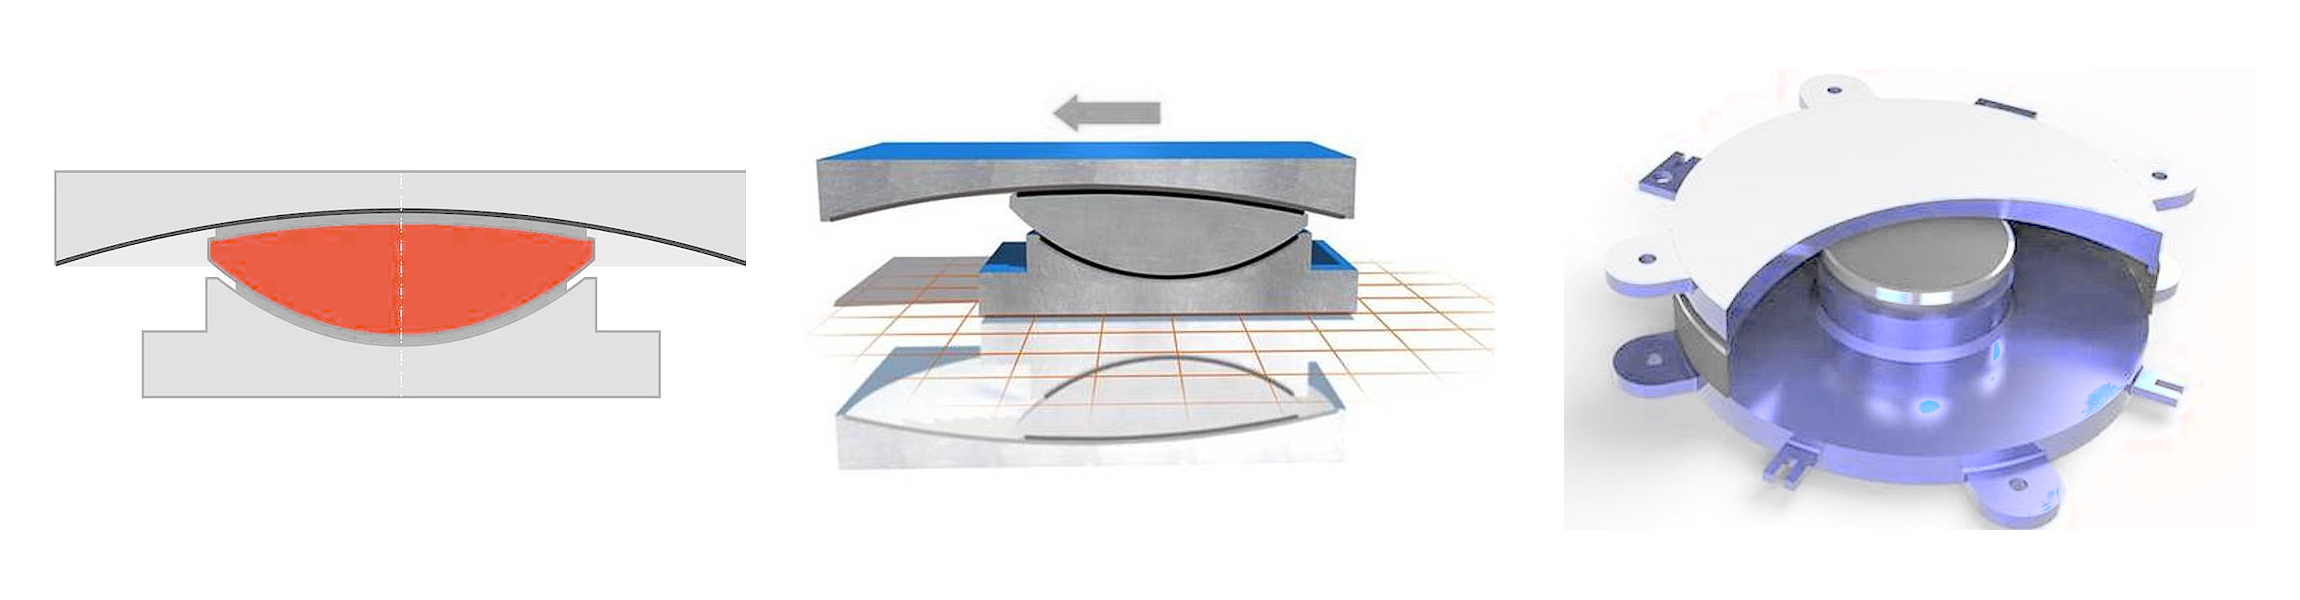
\includegraphics[width=0.9\textwidth]{maurer.png}
    \caption{Gleitpendelisolator [Maurer SE (maurer.eu)]}
\end{figure}

Die Reibung zwischen den Schnittstellen und somit die Dissipation kann eingestellt werden.
Bei einem zu hohen Reibkoeffizienten besteht jedoch die Gefahr, dass die Rückzentrierung nicht mehr gewährleistet werden kann, welche ein großer Vorteil der Gleitpendelisolatoren ist.
Zur Erhöhung der Dissipation können aber auch zusätzliche viskose Dämpfungselemente angeordnet werden.

\begin{figure}%
    \centering
    \subfloat[Gleitpendelisolator]{{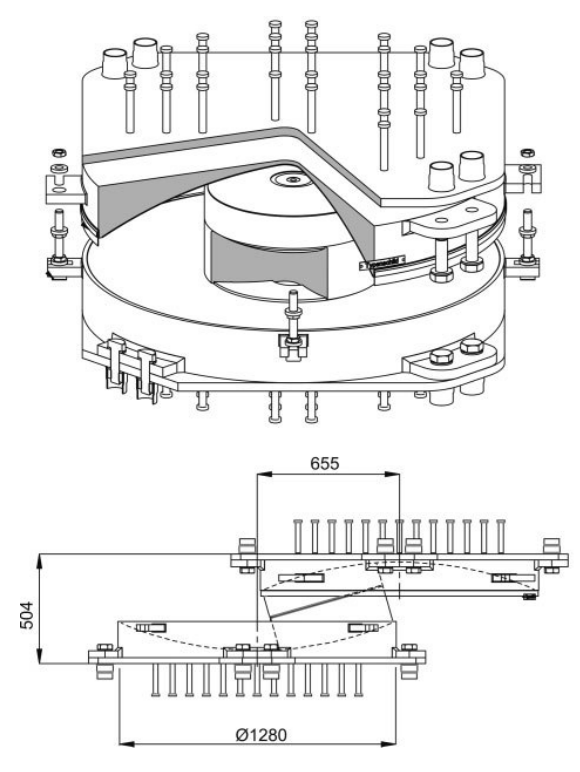
\includegraphics[width=0.45\linewidth]{Algerien_1.png} }}%
    \qquad
    \subfloat[Viskoser Hydraulikdämpfer]{{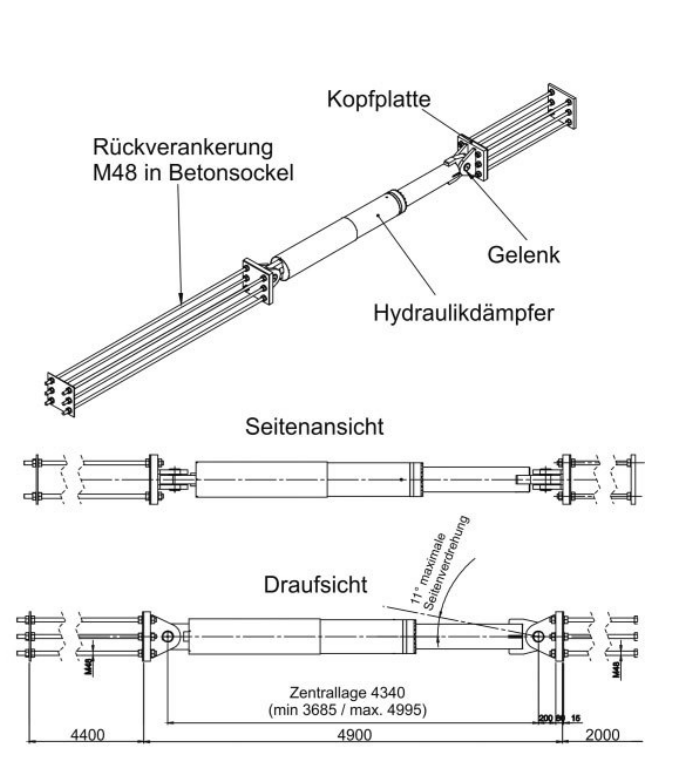
\includegraphics[width=0.45\linewidth]{Algerien_2.png} }}%
    \caption{Bauform der Iolatoren (a) und Dämpfer (b) der Großen Moschee von Algerien \cite{AKK}}%
\end{figure}

\begin{figure}
    \centering
    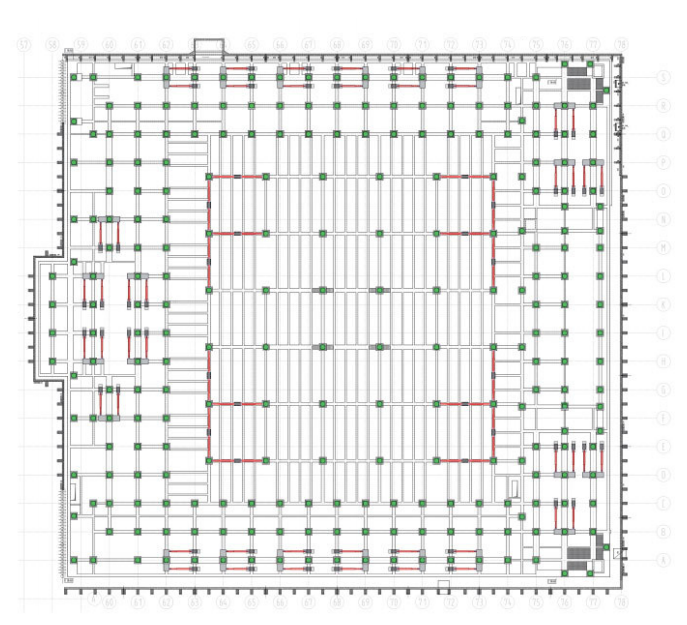
\includegraphics[width=0.9\textwidth]{Algerien_3.png}
    \caption{Verteilung der Iolatoren (grün) und Dämpfer (rot) im Grundriss \cite{AKK}}
\end{figure}

\pagebreak

\section{Funktionsweise}
\label{sec:funktion}

Isolatoren sind eine Ebene zwischen der Gründung und dem aufgehendem Bauwerk. Sie haben eine deutlich geringere Steifigkeit als die zu isolierende Struktur, wodurch zwar große Verschiebungen am Isolator auftreten, aber die Grundschwingzeit reduziert wird.
Die relativen Verschiebungen der Struktur werden verringert und somit die Beschleunigungen und ebenso die Trägheitskräfte der Massen reduziert.

\begin{figure}[h]
    \centering
    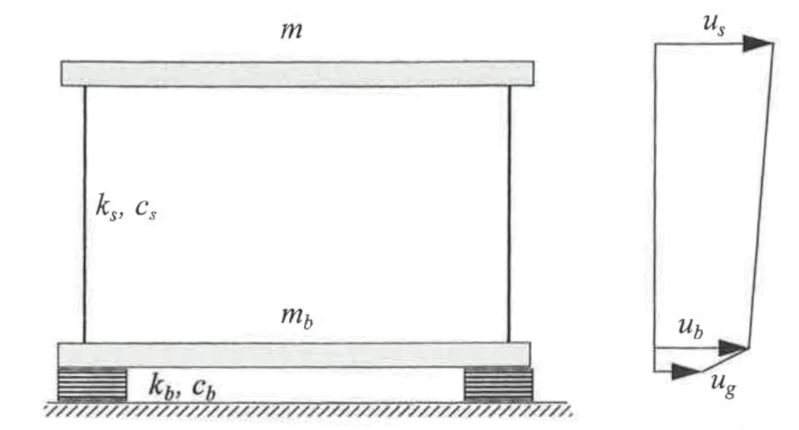
\includegraphics[width=0.9\textwidth]{Verschiebung_iso.png}
    \caption{Verteilung der Verschiebungen an einem isolierten System \cite{Kelly}}
\end{figure}

Die Dissipationsfähigkeit, Steifigkeit und Eigenfrequenz dieser Isolatoren kann über den Reibkoeffizienten, den Radius des Pendels und der Masse über dem Isolator beeinflusst werden.

\subsection{Dämpfung}
\label{sec:daempdung}


\begin{figure}[h]
    \centering
    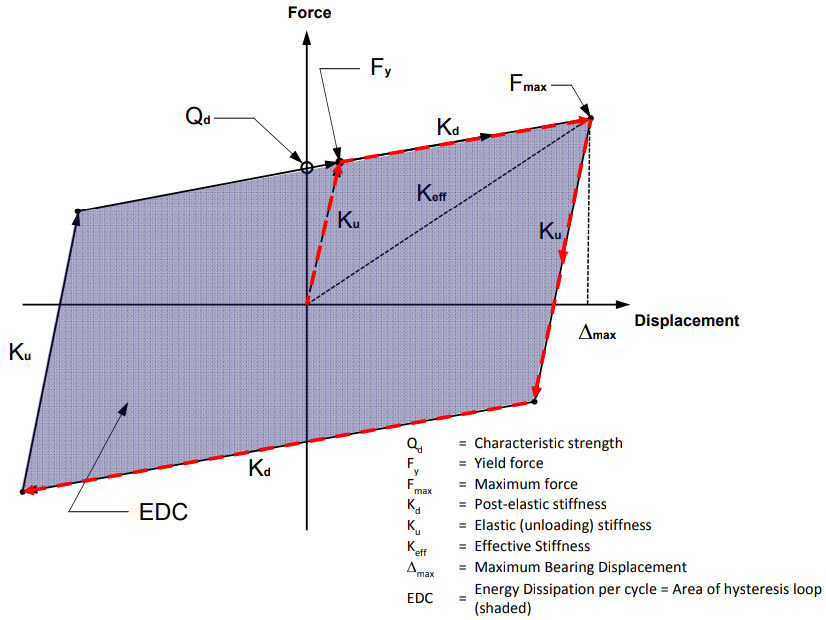
\includegraphics[width=0.9\textwidth]{Hysteresis.png}
    \caption{Hysterese-Zyklus [HDR Engineering Inc.]}
\end{figure}


\subsection{Steifigkeit}
\label{sec:steifigkeit}



Huber Hysterese Kruve 

Formeln Huber mit Umstellung nach Isemann

\pagebreak

\section{Schwierigkeiten bei der Vordimensionierung}
\label{sec:schwierigkeitenvordimensionierung}

Genaue Berechnung mit Zeitschrittverfahren
Grobe Vordimensionierung mit AWS

Schwierig weil Isolator mit modelliert werden muss


Optimierung, Bachmann, Pocanschi (426)

\pagebreak